\documentclass[a4paper, 11pt]{article}
\usepackage[utf8]{inputenc}

\usepackage[french]{babel}
\usepackage{graphicx} 
\usepackage{hyperref}
\usepackage{xcolor}
\usepackage{listings}
 \usepackage{enumitem}
\usepackage{amsmath} 
\usepackage{amsfonts}
\usepackage{hyperref}
\usepackage[left=2cm, right=2cm, bottom=3cm, top=3cm]{geometry}
\newcommand{\HRule}{\rule{\linewidth}{0.5mm}}
\us
\usepackage{natbib}
\usepackage{fancyhdr}
\pagestyle{fancy}
\fancyh{}
\rhead{\'{E}léments de processus stochastiques}
\lhead{Rapport du projet}
\rfoot{Année académique 2021-2022}
\lfoot{Université de Liège}

\begin{document}

\begin{titlepage}


\begin{center}
\includegraphics[scale = 0.35]{logo.jpg}\\
\vspace{1cm}
\textsc{\huge Université de Liège}\\[1.2cm]
\HRule \\[1cm]
\textsc{\LARGE MATH0488-1 : Eléments de processus stochastiques }\\[1cm]
{\Huge \bfseries Rapport du projet : \\ Méthodes de Monte Carlo par chaîne de Markov pour la détection de communautés dans un graphe}\\[1.4cm] 
\HRule \\[1cm]
    
\end{center}

\begin{minipage}{0.4\textwidth}
      \begin{flushleft} \large
        \emph{Auteurs : } \\
        Louis \textsc{Hogge}  S192814\\
        Hugo \textsc{Jacobs}  S193340 \\   
        Emilien \textsc{Leclerc} S190701 \\

      \end{flushleft}
\end{minipage}
\begin{minipage}{0.45\textwidth}
      \begin{flushright} \large
        \emph{Professeur : } P. \textsc{Geurts}\\
        \emph{Encadrants : } V. A.\textsc{ Huynh-Thu},\\ Y. \textsc{Claes}\\
        \emph{Année : } 2021-2022
      \end{flushright}
\end{minipage}
\end{titlepage}

\tableofcontents
\newpage
\listoffigures
\newpage

\section{Première partie : chaînes de Markov et algorithme MCMC}

\subsection{Chaîne de Markov}
\subsubsection{Question 1}
Dans un premier temps, on nous demande de calculer  numériquement $P(X_t=x)$, où $x=1,2,3,4$, pour des valeurs de $t$ croissantes, en supposant que : 
\begin{enumerate}
    \item l'état initial est tiré dans une loi uniforme discrète. On représente l'évolution de cette grandeur sur la figure \ref{unif} ci-dessous.
    \begin{figure}[h!]
        \centering
        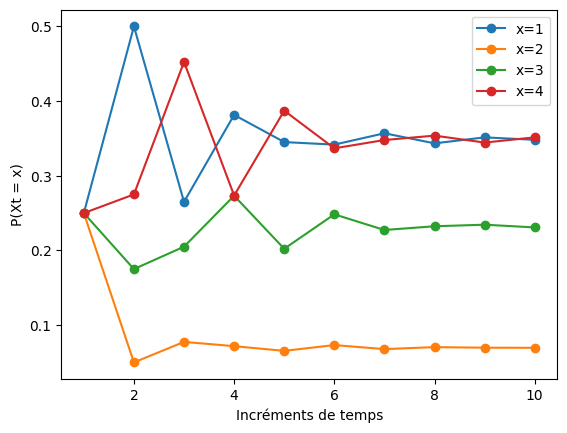
\includegraphics[scale=0.65]{evol_unif.png}
        \caption{Evolution de la première grandeur}
        \label{unif}
    \end{figure}
    \item l'état initial est toujours 3. L'évolution de cette grandeur est présentée à la figure \ref{trois} ci-dessous.
    \begin{figure}[h!]
        \centering
        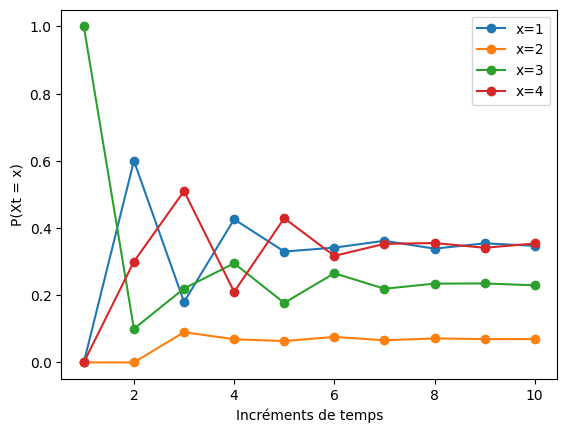
\includegraphics[scale=0.65]{evol_trois.png}
        \caption{Evolution de la deuxième grandeur}
        \label{trois}
    \end{figure}
\end{enumerate}

Sur la figure \ref{unif}, on remarque qu'au temps initial, la probabilité d'avoir les quatres états est la même. Cela est logique, puisque la distribution initiale est uniforme, donc la probabilité d'avoir les quatres états doit être la même. Pour les temps qui suivent, on peut cette fois remarquer que la probabilité d'avoir les états $x=1$ et $x=4$ croissent pour atteindre des valeurs similaires pour des temps grand. La probabilité d'avoir l'état $x=3$, bien que montrant des fluctuations, semble elle tendre vers la valeur qu'elle avait au début. Enfin, la probabilité d'avoir l'état $x=2$ décroît pour stagner pour des valeurs de temps grandes. Ces résultats s'expliquent sur base de la matrice de transition $Q$. Pour rappel, la matrice de transition des chaînes de Markov est définie comme
\begin{equation}
    Q_{ij}=P(X_{t+1}=j|X_t=i)
\end{equation}
et, dans ce cas-ci, cette matrice est donnée par
\begin{equation}
    Q=\begin{pmatrix}
    0 & 0.1 & 0.1 & 0.8 \\
    1 & 0 & 0 & 0 \\
    0.6 & 0 & 0.1 & 0.3 \\
    0.4 & 0.1 & 0.5 & 0 \\ 
    \end{pmatrix}
\end{equation}
On remarque alors, sur cette matrice, que si l'on est dans les états $x=1,3,4$ au temps $t$, la probabilité d'être dans l'état $x=2$ au temps $t+1$ est toujours égale à 0,1. Par conséquent, il est normal que la probabilité d'être dans l'état $x=2$ au temps $t+1$ soit faible. Ensuite, on peut remarquer que la probabilité d'être à $t+1$ dans l'état $x=1$ est très élevée, et peu importe l'état au temps $t$, ce qui explique que la probabilité d'avoir l'état $x=1$ est assez importante au fil du temps. Ce constat peut aussi être fait pour l'état $x=4$. Enfin, la probabilité d'être en $t+1$ dans l'état $x=3$ semble intermédiaire, ce qui se traduit également sur la figure \ref{unif}.\\

Sur la figure \ref{trois}, on remarque que cette fois qu'au temps initial, comme attendu, la probabilité d'avoir l'état $x=3$ vaut 1 et les autres sont nulles. Ensuite, lorsque le temps grandit, les probabilités d'avoir chaque état semble tendre vers les mêmes valeurs qu'on peut observer sur la figure \ref{unif}. Cela s'explique de manière similaire, à l'aide de la matrice de transition.
\newpage
 \subsubsection{Question 2}
 De ces résultats, on déduit assez aisément la distribution stationnaire $\pi_\infty$ de la chaîne de Markov, définie par 
 \begin{equation}
     [\pi_\infty]_j=lim_{t\rightarrow \infty} P(X_t=j)
 \end{equation}
Cette distribution représente en fait les probabilités d'avoir chaque état, lors d'un incrément de temps infini. On a vu sur les figures \ref{unif} et \ref{trois} que ces valeurs étaient stables pour des incréments de temps grandissant. Cela correspond donc, par conséquent, à ces valeurs. On représente cette distribution sur la figure \ref{fig:dist_inf}.
\begin{figure}[h!]
    \centering
    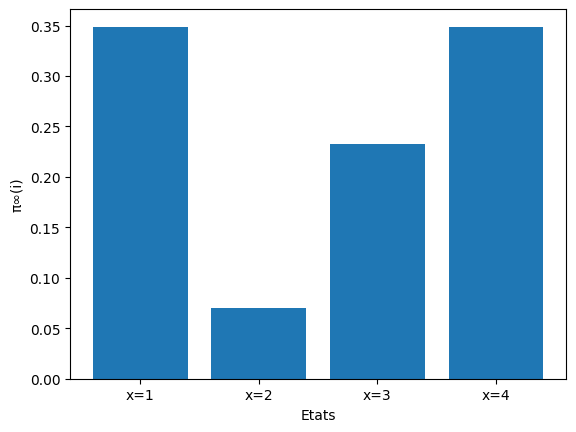
\includegraphics[scale=0.6]{pi_inf.png}
    \caption{Distribution stationnaire $\pi_\infty$ de la chaîne de Markov}
    \label{fig:dist_inf}
\end{figure}
\newpage
\subsubsection{Question 3}
Par après, on va générer des chaînes de Markov de longueur $T$ variable. Pour chaque longueur $T$, on calcule la proportion de chaque état dans la chaîne. Sur la figure \ref{fig:evol_prop} ci-dessous, on représente la proportion de chaque état, pour chaque taille de chaîne de Markov.
\begin{figure}[h!]
    \centering
    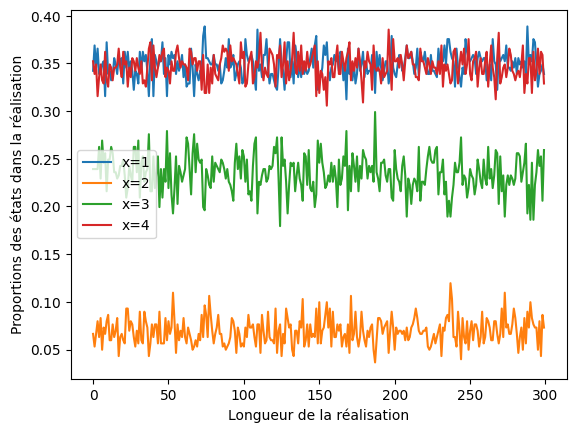
\includegraphics[scale=1]{evol_states.png}
    \caption{Evolution de la proportion de chaque état dans des chaînes de Markov de taille variable}
    \label{fig:evol_prop}
\end{figure}\\

Les résultats de cette figure semblent relativement clairs. En effet, il est aisé de se rendre compte que, pour un état, la proportion de celui-ci dans la chaîne de Markov semble toujours plus ou moins égale, et ce pour chaque état. De plus, ces proportions sont relativement égales aux valeurs que donnait la distribution stationnaire $\pi_\infty$ à chaque état.
\subsubsection{Question 4}
De cette expérience, on conclut assez aisément que les probabilités de retrouver chaque état au temps $t+1$ tendent vers une valeur constante, et ce quelle que soit la taille de la chaîne de Markov. Cette propriété se traduit par le fait que la chaîne de Markov étudiée ici possède une distribution stationnaire, soit que 
$$\pi_s=\pi_s Q$$
En d'autres termes, on peut augmenter la taille de la chaîne de Markov à l'infini sans que la probabilité de trouver un état ou un autre au temps $t+1$ soit modifiée. 
\newpage
\subsection{Méthode MCMC : analyse théorique dans le cas fini}
\subsubsection{Question 1}
Dans un premier temps, il nous faut démontrer que, étant donné une matrice de transition $Q$ et une distribution $\pi_0$ d'une chaîne de Markov invariante dans le temps qui satisfont les équations de balance détaillées, soit que
\begin{equation}
    \forall i,j \in { 1,...N} : \pi_0(i) [ Q]_{i,j}=\pi_0(j) [ Q,]_{j,i}
    \label{1}
\end{equation}
que $\pi_0$ est une distribution  stationnaire d'une chaîne de Markov.\\
Pour rappel, la matrice de transition, $Q$, de taille $n$, est définie comme étant
\begin{equation}
Q=
    \begin{pmatrix}
    P(X_1=x_1|X_0=x_1) & ... & P(X_1=x_n|X_0=x_1)\\
    ... & P(X_1=x_j|X_0=x_i) & ...\\
    P(X_1=x_1|X_0=x_n) & ... & P(X_1=x_n|X_0=x_n)\\
    \end{pmatrix}
    \label{2}
\end{equation}
alors que, la distribution $\pi_0$, de taille $n$, d'une chaîne de Markov est définie comme étant:
\begin{equation}
    \pi_0=
    \begin{pmatrix}
    P(X_0=x_1) ...  P(X_0=x_k) .... P(X_0=x_n)
    \end{pmatrix}
    \label{3}
    \end{equation}
De  plus, nous savons également que la chaîne de Markov est invariante, ce qui signifie que 
$$Q_0=Q_1=Q_2=...=Q_n=Q$$
De part les équations de balance détaillées qui ont été explicitée à l'équation \ref{1}, nous obtenons, en utilisant les résultats explicités aux équations \ref{2} et \ref{3} 
\begin{equation}
    P(X_0=x_i)P(X_1=x_j|X_0=x_i)=P(X_0=x_j)P(X_1=x_i|X_0=x_j)
\end{equation}
En faisant usage de la loi de Bayes, il vient
\begin{equation}
    P(X_0=x_i) \frac{P(X_1=x_j,X_0=x_i)}{P(X_0=x_i)}=P(X_0=x_j) \frac{P(X_1=x_j,X_0=x_i)}{P(X_0=x_j)}
\end{equation}
Soit, après simplification, 
\begin{equation}
    P(X_1=x_j,X_0=x_i)=P(X_1=x_j,X_0=x_i), \forall i,j \in [1,...n]
    \label{6}
\end{equation}
Nous devons démontrer que $\pi_0$ est une distribution stationnaire, soit que, $\pi_1=\pi_0$. Or, nous savons également que, par invariance, $\pi_1=Q\pi_0$. En usant ce qui a été explicité aux équations \ref{2} et \ref{3}, il vient aisément que
\begin{equation}
    P(X_1=x_j)=\sum^n_{k=1} P(X_0=x_k)P(X_1=x_k|X_0=x_k)
\end{equation}
Soit, en utilisant la loi de Bayes
\begin{equation}
    P(X_1=x_j)=\sum^n_{k=1} P(X_0=x_k)\frac{P(X_1=x_k,X_0=x_k)}{P(X_0=x_k)}
\end{equation}
Ce qui donne, après simplification
\begin{equation}
    P(X_1=x_j)=\sum^n_{k=1}P(X_1=x_k,X_0=x_k)
\end{equation}
En usant ce qui a été vu à l'équation \ref{6}, il vient alors
\begin{equation}
    P(X_1=x_j)=\sum^n_{k=1}P(X_1=x_k,X_0=x_k)=\sum^n_{k=1}P(X_1=x_k,X_0=x_j)
\end{equation}
Il vient alors aisément que
\begin{equation}
    P(X_1=x_j)=P(X_0=x_j)
\end{equation}
ce qui signifie que $\pi_0=\pi_1$, et donc que $\pi_0$ est une distribution stationnaire, qui est ce qu'il fallait démontrer. Cette distribution peut être considérée comme unique si la matrice de transition $Q$ qui définit cette chaîne est irréductible.
\subsubsection{Question 2}\label{Q122}
Dans le cas d'une variable aléatoire $X$ discrète, on cherche à démontrer que l'application de l'algorithme de Metropolis-Hastings, en remplaçant $p_X$ par une fonction $f$ telle que $\forall x, f(x)=cp_X (x)$, où $c$ est une constante, génère une chaîne de Markov dont les équations de balance détaillée sont satisfaites avec $p_X$ comme distribution stationnaire. De manière générale, la probabilité d'acceptation de l'algorithme de Metropolis-Hastings est donnée par


\begin{equation}
    \alpha (y^{(t)},x^{(t-1)})=min \left( 1 , \frac{f (y^{(t)})}{f (x^{(t-1)})} \frac{q(x^{(t-1)}|y^{(t)})}{q(y^{(t)}|x^{(t-1)})} \right)
\end{equation}
ce qui reviens à 
\begin{equation}
    \alpha (y^{(t)},x^{(t-1)})=min \left( 1 , \frac{p_X (y^{(t)})}{p_X (x^{(t-1)})} \frac{q(x^{(t-1)}|y^{(t)})}{q(y^{(t)}|x^{(t-1)})} \right)
\end{equation}
si l'on suppose que
$$M=\frac{p_X (y^{(t)})}{p_X (x^{(t-1)})} \frac{q(x^{(t-1)}|y^{(t)})}{q(y^{(t)}|x^{(t-1)})}$$
Deux cas distincts apparaissent
\begin{itemize}[label=\textbullet]
    \item \underline{$M\ge 1$}
    Dans ce cas-ci, on a alors 
    $$\alpha (y^{(t)},x^{(t-1)})=1$$
    Ce faisant, on peut alors aussi déterminer que
    $$\alpha (x^{(t-1)},y^{(t)})=min(1,\frac{1}{M})$$
    et, en utilisant la condition,
    $$\alpha (x^{(t-1)},y^{(t)})=\frac{p_X (x^{(t-1)})}{p_X (y^{(t)})} \frac{q(y^{(t)}|x^{(t-1)})}{q(x^{(t-1)}|y^{(t)})}$$ 
    \item \underline{$M< 1$}
    Dans ce second cas, on obtient que
    $$\alpha (y^{(t)},x^{(t-1)})=M=\frac{p_X (y^{(t)})}{p_X (x^{(t-1)})} \frac{q(x^{(t-1)}|y^{(t)})}{q(y^{(t)}|x^{(t-1)})}$$
    De plus, de manière similaire au premier cas, on a 
    $$\alpha (x^{(t-1)},y^{(t)})=1$$
    \end{itemize}
    Les deux cas peuvent mener au même résultat, soit que
    \begin{equation}
        \alpha (y^{(t)},x^{(t-1)}) p_X (x^{(t-1)}) q(y^{(t)}|x^{(t-1)})=\alpha (x^{(t-1)},y^{(t)}) p_X (y^{(t)}) q(x^{(t-1)}|y^{(t)})
    \end{equation}
    Or, selon la loi de Bayes, il vient
    $$ \alpha (x^{(t-1)},y^{(t)}) q(y^{(t)}|x^{(t-1)})=q(x^{(t-1)}|y^{(t)})=Q(x^{(t-1)},y^{(t)})$$
    On obtient alors
    \begin{equation}
    p_X (x^{(t-1)}) Q(x^{(t-1)},y^{(t)})=p_X (y^{(t)}) Q(y^{(t)},x^{(t-1)})
    \end{equation}
    qui demeure une équation de balance détaillée, qui est donc satisfaite par la chaîne de Markov générée par l'algorithme de Metropolis-Hastings, qui est ce qu'on cherchait à démontrer. Une autre condition que doit respecter la chaîne de Markov doit respecter pour que cet algorithme fonctionne est que la probabilité de proposer une certaine valeur $y$ ne soit jamais nulle, soit que 
    $$\forall x,y; q(y^{(t)}|x^{(t-1)})\ne 0$$
    Cette propriété de la fonction de proposition est appelée l'irréductibilité  de la fonction de proposition. Elle signifie qu'à tout temps, la probabilité d'atteindre un état à partir de n'importe quel état est non-nulle, c'est-à-dire qu'il est possible d'atteindre n'importe quel état à partir d'un état. De plus, il apparaît que cette fonction de proposition doit également être apériodique, soit que le chaîne sera toujours différente si on recommence celle-ci.
    \newpage
\subsection{Méthode MCMC : Illustration sur un exemple simple}
\subsubsection{Question 1}
On souhaite appliquer l'algorithme de Metropolis-Hastings pour échantillonner des valeurs de la loi binomiale suivante:
\begin{equation}
    P(X=k)=C_K^k p^k (1-p)^{K-k}
    \label{distrib}
\end{equation}
où $p$ et $K$ sont des paramètres, donnés par $p=0.3$ et $K=10$ et $k\in \{0,1,...K\}$. Pour ce faire, on souhaite,utiliser la distribution de proposition suivante, où $r\in ]0,1[$,
\begin{equation}
    q(y|x) = \left\{
    \begin{array}{ll}
        r & \mbox{si } x=0 ~\mbox{et } y=0,\\
        (1-r) & \mbox{si } x=K~\mbox{et }y=K,\\
        r   & \mbox{si } 0 < x \le K~\mbox{et }y=x-1,\\
        (1-r) & \mbox{si } 0 \le x < K~\mbox{et } y=x+1,\\
        0 & \mbox{sinon.}
    \end{array}
\right.
\label{q}
\end{equation}
Ici, on cherche à démontrer que cette distribution de proposition ($q(y|x)$) de l'algorithme de Metropolis-Hastings générera effectivement des échantillons selon la distribution $p_X(x)$ explicitée ci-dessus. On a démontré à la section \ref{Q122} que pour que ce soit le cas, il faut que
\begin{equation}
    p_X (x^{(t-1)}) Q(x^{(t-1)},y^{(t)})=p_X (y^{(t)}) Q(y^{(t)},x^{(t-1)})
\end{equation}
Dès lors, ici, on va chercher à démontrer que 
\begin{equation}
    p_X(x) q(x|y)=p_X(y) q(y|x)
    \label{22}
\end{equation}
Or, on a vu dans la section \ref{Q122} que pour que cette égalité soit valable, il faut que la fonction de proposition soit irréductible et apériodique.\\
Premièrement, cette fonction de proposition est irréductible, c'est à-dire que $$q(y^{(t)}|x^{(t-1)}) \ne 0, \forall x,y $$
En effet, en observant l'expression de la fonction de proposition, à l'équation \ref{q}, on remarque que, quel que soit le $x^{(t-1)}$, la probabilité d'atteindre $y^{(t)}$ est non-nulle (puisque états sont entiers). On en déduis assez aisément que cette fonction est irréductible. De plus, il fallait que cette fonction soit apériodique. C

\newpage
\subsubsection{Question 2}\label{132}
On peut ensuite analyser les échantillons obtenus pour $r=0,1$ et $r=0,5$, lorsque l'on applique l'algorithme de Metropolis-Hastings à la fonction de proposition obtenue. Pour analyser ceux-ci, on représente l'évolution des moyennes et des variances des échantillons produits par l'algorithme en fonction de la taille de ceux-ci. On commencera par les moyennes. La distribution théorique, celle dont on souhaite générer des valeurs par Metropolis Hastings est une loi binomiale, donnée à l'équation \ref{distrib}. L'espérance de cette loi théorique est alors donnée par
\begin{equation}
    E(X)=np=10\times 0.3=3
\end{equation}
Les chaînes obtenues par l'algorithme devraient avoir une moyenne qui s'approche de cette valeur. On représente à la figure \ref{mean} l'évolution de la moyenne des échantillons en fonction de la taille des échantillons.

\begin{figure}[h!]
    \centering
    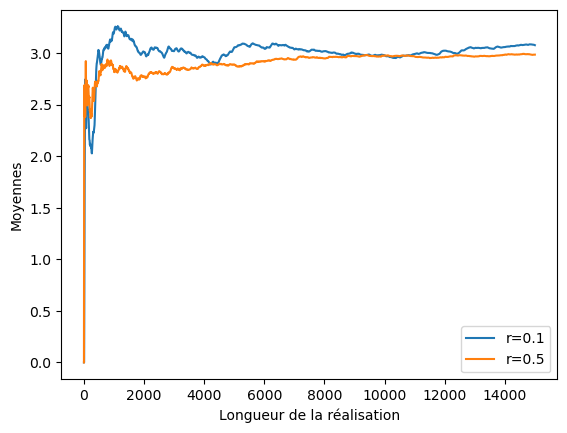
\includegraphics[scale=1]{mean.png}
    \caption{Comparaison des moyennes des échantillons obtenus par MH en fonction de la longueur de la réalisation, avec $r=0,1$ et $r=0,5$}
    \label{mean}
\end{figure}\\

On remarque que, pour les deux valeurs de $r$, pour des tailles d'échantillons grandes, la moyenne de ceux-ci semble converger vers une valeur qui est approximativement égale à celle de la moyenne théorique. De plus, on remarque que celle-ci converge plus vite vers la bonne valeur lorsque $r=0,5$.\\

Ensuite, on peut étudier la convergence des variances des échantillons. La variance de la loi théorique binomiale est donnée par
\begin{equation}
    Var(X)=n\times p \times  (1-p)=10\times 0,3 \times 0,7=2,1
\end{equation}
On représente sur la figure \ref{var} l'évolution de la variance pour les deux valeurs de $r$,  en fonction de la taille des échantillons. 

\begin{figure}[h!]
    \centering
    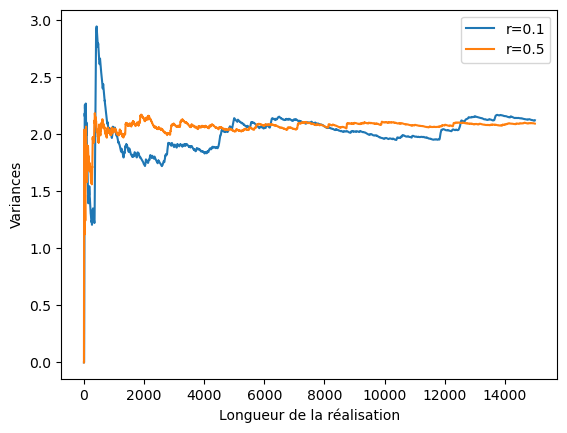
\includegraphics[scale=1]{var.png}
    \caption{Comparaison des variances des échantillons obtenus par MH en fonction de la longueur de la réalisation, avec $r=0,1$ et $r=0,5$}
    \label{var}
\end{figure}\\

Les résultats de cette figure corroborent à ceux obtenus pour la moyenne. En effet, on remarque que pour des grandes tailles d'échantillons, les variances tendent vers la valeur théorique. La variance de $r=0,5$ converge à nouveau plus vite vers la bonne valeur.
\newpage
\subsubsection{Question 3}
Enfin, on peut également tracer l'histogramme de la fréquence d'apparition de chaque valeur, et ce pour les deux valeurs de $r$ qui ont été utilisée jusqu'ici : $r=0,1$ et $r=0,5$. Pour chacune de ces valeurs, on comparera le résultat obtenu à l'histogramme que donnerait la distribution binomiale théorique. La figure \ref{fig:hist1} ci-dessous présente l'histogramme pour $r=0,1$.
\begin{figure}[h!]
    \centering
    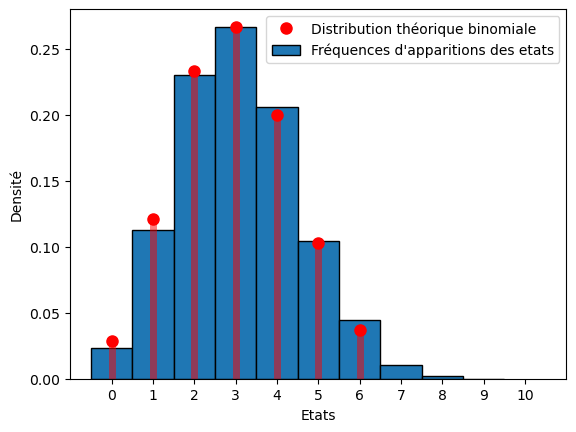
\includegraphics[scale=0.8]{hist_r_01.png}
    \caption{Histogramme des fréquences d'apparition, pour $r=0,1$}
    \label{fig:hist1}
\end{figure}\\

Cette figure montre que, pour $r=0,1$, l'algorithme de Metropolis-Hastings fournit un échantillon qui se rapproche plus ou moins de la distribution théorique attendue. En effet, les fréquences d'apparition pour chaque états se rapproche assez de celle d'une loi binomiale théorique.\\

Ensuite, on peut analyser cette comparaison, mais cette fois lorsque $r=0,5$. Cette comparaison est faite à la figure \ref{fig:hist2}. \\

On remarque que, comme lorsque $r=0,1$, les distributions empiriques, obtenues par l'algorithme de Metropolis-Hastings, et théoriques semble présenter des formes plus ou moins similaires. De plus, on remarque que la distribution empirique obtenue pour la fonction de proposition, lorsque $r=0,5$, semble être plus précise, mieux épouser la distribution théorique que lorsque $r=0,1$. On avait déjà observé à la section \ref{132} que, lorsque $r=0,5$, les résultats semblaient être plus précis.

\begin{figure}[h!]
    \centering
    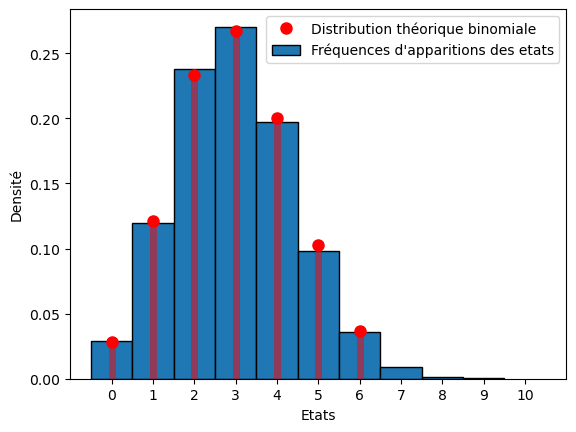
\includegraphics[scale=0.8]{hist_r_05.png}
    \caption{Histogramme des fréquences d'apparition, pour $r=0,5$}
    \label{fig:hist2}
\end{figure}
\newpage
\section{Deuxième partie : détection de communautés dans un graphe par méthode MCMC}
La deuxième partie de ce projet cherchera à implémenter un code capable de détecter des communautés dans un graphe donné. Pour ce faire, on utilisera la méthode MCMC, c'est-à-dire Monte-Carlo par chaîne de Markov. Ceci utilisera l'algorithme de Metropolis-Hastings. On commencera par une étude théorique de cet algorithme, avant de réaliser une analyse expérimentale, puis appliquer celui-ci à des graphes plus conséquent, ce qui est la finalité de ce projet.
\subsection{Étude théorique}
Dans un premier temps, on étudiera l'implémentation de manière théorique.
\subsubsection{Question 1}\label{211}
Pour commencer, on cherche à expliciter la distribution $P(x|G)$ pour deux modèles différents.
\begin{enumerate}
    \item \underline{Modèle Général : $SBM (N,K,p,W)$}\\\\
    
    Par une simple utilisation de la loi de Bayes, on obtient aisément
    \begin{equation}
        P(x|G)=\frac{P(G|x)P(x)}{P(G)}
        \label{Bayes1}
    \end{equation}
    Dans cette égalité, on connaît l'entièreté des termes qui constituent le second membre. On a, d'abord,
    \begin{equation}
        P(x)=P(X=x)=\prod^N_{i=1}p_{X_i}
    \end{equation}
    Par la suite, on a aussi
    \begin{equation}
        P(G|x)=\prod_{1\le i \le j \le K} W_{i,j}^{d_{i,j}} (1-W_{i,j})^{\lnot ~
        ~d_{i,j}}
        \label{eq:24}
    \end{equation}
    L'équation  \ref{eq:24} contient des termes qu'il est important de définir. Plus particulièrement, on a
    \begin{itemize}
        \item $N$ est le nombre de noeuds du graphe,
        \item $K$ est le nombre de communautés du graphe,
        \item $W_{i,j}$ est la probabilité de connexion entre le noeud $x_i$ et le noeud $x_j$,
        \item $d_{i,j}$ est le nombre d'arêtes entre la communauté contenant $x_i$ et celle contenant $x_j$. Pour conséquent, $\lnot d_{i,j}$ est l'inverse de $d_{i,j}$, soit la différence entre le nombre maximal d'arêtes possibles entre les deux communautés et le nombre d'arêtes qu'il y a réellement.
    \end{itemize}
    Enfin, on sait également que
    \begin{equation}
        P(G)=\sum_x P(G|x) P(x)
    \end{equation}
    En injectant l'ensemble de ces résultats dans l'équation \ref{Bayes1}, on a alors
    \begin{equation}
        P(x|G)=\frac{\prod_{1\le i \le j \le K} W_{i,j}^{d_{i,j}} (1-W_{i,j})^{\lnot ~
        ~d_{i,j}} \times \prod^N_{i=1}p_{X_i} }{\sum_x (\prod_{1\le i \le j \le K} W_{i,j}^{d_{i,j}} (1-W_{i,j})^{\lnot ~
        ~d_{i,j}} \times \prod^N_{i=1}p_{X_i}) }
    \end{equation}
    \\
    \item \underline{Modèle Simplifié : $SBM(N,K,p,A,B)$}\\
    
    Dans le cas du modèle simplifié, on sait qu'on a
    $$ W_{i,i}=A;~\forall i \mbox{ et } W_{i,j}=B;~\foralli,j~:~i\ne j$$
    L'équation \ref{eq:24} devient alors
    \begin{equation}
        \begin{split}
            P(G|x)=\prod_{1\le i \le j \le K} W_{i,j}^{d_{i,j}} (1-W_{i,j})^{\lnot ~
        ~d_{i,j}}\\
        \Longleftrightarrow P(G|x)=\prod^K_{i=1} W_{i,i}^{d_{i,i} }(1-W_{i,i})^{\lnot d_{i,i}} . \prod_{1\le i \le j \le K, i\ne j} W_{i,j}^{d_{i,j}} (1-W_{i,j})^{\lnot ~
        ~d_{i,j}}\\
        \Longleftrightarrow P(G|x)=\prod^K_{i=1} A^{d_{i,i} }(1-A)^{\lnot d_{i,i}} . \prod_{1\le i \le j \le K, i\ne j} B^{d_{i,j}} (1-B)^{\lnot ~
        ~d_{i,j}}\\
        \end{split}
        \label{demoo}
    \end{equation}
    On peut chercher à déterminer la valeur de l'inverse de $d_{i,i}$, $\lnot d_{i,i}$. On obtient, si $nb~x_i$ est le nombre de noeuds appartenant à la communauté $i$
    $$\lnot d_{i,i}=\sum^{nb~x_i}_{i=1} nb~x_i-i-d_{i,i}= nb~x_i^2-\sum_{i=1}^{nb~x_i} i-d_{i,i}=nb~x_i- \frac{nb~x_i (nb~x_i+1)}{2}-d_{i,i}$$
    On obtient alors, si on note $\Omega_i (x)= nb~x_i$
    \begin{equation}
        \lnot d_{i,i}=\lvert \Omega_i(x)\rvert \frac{(\lvert \Omega_i(x) \rvert -1)}{2}-d_{i,i}
    \end{equation}
    Et, en utilisant le même raisonnement, on obtient alors
    \begin{equation}
        \lnot d_{i,j}=nb~x_i \times nb~x_j -d_{i,j}=\lvert \Omega_i(x)\rvert \lvert \Omega_j (x) \rvert -d_{i,j}
    \end{equation}
    L'équation \ref{demoo} devient alors
    \begin{equation}
        P(G|x)=\prod^K_{i=1} (A^{d_{i,i}}-A^{\lvert \Omega_i(x)\rvert \frac{(\lvert \Omega_i(x) \rvert -1)}{2}}) \prod_{1\le i \le j \le K, i\ne j} (B^{d_{i,j}}-B^{\lvert \Omega_i(x)\rvert \lvert \Omega_j (x) \rvert})
    \end{equation}
    La distribution $P(x)$, quant à elle, peut être réécrite comme suit
    \begin{equation}
        P(x)=\prod^K_{i=1} p_i^{\lvert \Omega_i(x) \rvert}
    \end{equation}
    Finalement, en injectant tout ces nouveaux résultats dans l'équation \ref{Bayes1}, on obtient que
    \begin{equation}
        P(x|G)=\frac{\prod^K_{i=1} (A^{d_{i,i}}-A^{\lvert \Omega_i(x)\rvert \frac{(\lvert \Omega_i(x) \rvert -1)}{2}}) \prod_{1\le i \le j \le K, i\ne j} (B^{d_{i,j}}-B^{\lvert \Omega_i(x)\rvert \lvert \Omega_j (x) \rvert}). \prod^K_{i=1} p_i^{\lvert \Omega_i(x) \rvert}}{\sum_{x_k} (\prod^K_{i=1} (A^{d_{x_k,i,i}}-A^{\lvert \Omega_i(x_k)\rvert \frac{(\lvert \Omega_i(x_k) \rvert -1)}{2}}) \prod_{1\le i \le j \le K, i\ne j} (B^{d_{x_k,i,j}}-B^{\lvert \Omega_i(x_k)\rvert \lvert \Omega_j (x_k) \rvert}). \prod^K_{i=1} p_i^{\lvert \Omega_i(x_k) \rvert})}
        
        %\frac{\prod_{i=1}^K A^{d_{i,i}} (1-A)^{\lvert \Omega_i(x)\rvert \frac{(\lvert \Omega_i(x) \rvert -1)}{2}}. \prod_{1\le i \le j \le K, i\ne j} B^{d_{i,j}} (1-B)^{\lvert \Omega_i(x)\rvert \lvert \Omega_j (x) \rvert}). \prod^K_{i=1} p_i^{\lvert \Omega_i(x) \rvert}}{\sum_x (\prod_{i=1}^K A^{d_{i,i}} (1-A)^{\lvert \Omega_i(x)\rvert \frac{(\lvert \Omega_i(x) \rvert -1)}{2}}. \prod_{1\le i \le j \le K, i\ne j} B^{d_{i,j}} (1-B)^{\lvert \Omega_i(x)\rvert \lvert \Omega_j (x) \rvert}). \prod^K_{i=1} p_i^{\lvert \Omega_i(x) \rvert})}
    \end{equation}
    
    \end{enumerate}
\subsubsection{Question 2}
Le but ici est de partitionner le graphe $G$ étudié en communautés. Une première idée pour obtenir ces communautés serait de générer tout les vecteurs de communauté possibles. Un vecteur de communauté est un vecteur contenant pour chaque noeud la communauté à laquelle il appartient. Avec tous les vecteurs ainsi créés, on pourrait chercher le vecteur de communauté $x$ qui maximiserait $P(x|G)$, soit le vecteur le plus proche de la vraie répartition des communautés.\\

En pratique, cette méthode apparaît trop compliqué à mettre en oeuvre pour des graphes à $N$ noeuds, si $N$ est grand. En effet, le nombre de vecteur de communautés disponibles serait de l'ordre de $N!$, soit un nombre infiniment trop grand pour une résolution numérique.\\

La solution alors trouvée est d'utiliser l'algorithme de Metropolis-Hastings, pour lequel une grande valeur de $N$ ne poserait pas problème. Celui-ci consiste à échantillonner des solutions $x$ candidates selon la distribution $P(x|G)$, en suivant une distribution de proposition $q_s$. Ensuite, il suffira de choisir le vecteur de communauté $x$ qui maximise $P(x|G)$. L'usage de cet algorithme permettra de ne pas devoir tester toutes les vecteurs de communautés possibles, mais seulement ceux qui sont candidats, selon la distribution $P(x|G)$, et dès lors, la résolution numérique est possible.
\subsubsection{Question 3}
On souhaite s'assurer que la distribution $q_s$ proposée ici pour l'algorithme de Metropolis-Hastings est valide. On a vu à la section\ref{Q122} que pour que ce soit le cas, il fallait que la fonction de proposition soit irréductible et apériodique. Ici, on propose $q_s$, qui est en fait de choisir aléatoirement un noeud dans une communauté et de le changer. De part le processus aléatoire décrit ici, il semble qu'à la fois l'irréductibilité et l'apériodicité de la fonction de distribution sont assurées. Cette fonction de distribution est donc valide. 

\subsubsection{Question 4}
On peut également s'intéresser maintenant à la probabilité d'acceptation de l'algorithme de Metropolis-Hastings. Pour rappel, celle-ci est donnée par, dans ce cas-ci,
\begin{equation}
    \alpha(y^{(t)}, x^{(t-1)})=min \left( 1,  \frac{P(G|y^{(t)})}{P(G|x^{(t-1)})} \frac{P(y^{(t)})}{P(x^{(t-1)})} \right)
\end{equation}
Avec les expressions qui ont été déterminée à la section \ref{211}, on obtient alors aisément que
\begin{equation}
    \alpha(y^{(t)}, x^{(t-1)})= min (1, G)
\end{equation}
où $G$ est donné par 
\begin{equation}
    G=\prod^K_{i=1} \left[ \frac{A^{dy_{i,i}}-A^{\lvert \Omega_i(y^{(t)})\rvert \frac{(\lvert \Omega_i(y^{(t)}) \rvert -1)}{2}}}{A^{dx_{i,i}}-A^{\lvert \Omega_i(x^{(t-1)})\rvert \frac{(\lvert \Omega_i(x^{(t-1)}) \rvert -1)}{2}}} \right]. \prod_{1\le i \le j \le K, i\ne j} \left[ \frac{A^{dy_{i,i}}-A^{\lvert \Omega_i(y^{(t)})\rvert  \lvert \Omega_j(y^{(t)})\rvert}}{A^{dx_{i,i}}-A^{\lvert \Omega_i(x^{(t-1)})\rvert \lvert \Omega_j(x^{(t-1)})\rvert}} \right]. \prod^K_{i=1} p_i^{ \lvert \frac{\Omega_i(y^{(t)}}{\Omega_i(x^{(t-1)})} \rvert}
\end{equation}
\newpage
\subsection{Analyse expérimentale} 
On commence par une analyse expérimentale de l'algorithme de Metropolis-Hastings avec l'identification des communautés en fonction des paramètres $A$ et $B$ ($A=a/N$ et $B=b/N$). On supposera deux communautés $(K=2)$ et une distribution de communautés $p=(1/2,1/2)$.
\subsubsection{Question 1}\label{221}
Premièrement, on fixe le degré moyen $\frac{a+b}{2}$ à $20$. On souhaite étudier l'évolution de la concordance moyenne en fonction du rapport $b/a$, qui varie dans $[0,1]$ (donc $a>b$). Elle est donnée par
\begin{equation}
    E_{(x^*,G)\sim (N,2,p,a/N,b/N)}\left\{ E_{P(x|G)} \left\{A(x^*,x) \right\} \right\}
\end{equation}
Afin d'étudier cette concordance, pour chaque valeur de $a \in [21,39]$ et sa valeur de $b \in [19,1]$ correspondante, on génère 10 graphes de tailles 1000x1000 et leurs vecteurs de communautés associés à l'aide d'un générateur de graphes selon le modèle SBM. Sur chacun des graphes générés, on applique l'algorithme de Metropolis-Hastings avec 100 000 itérations. Cet algorithme va fournir une estimation du vecteur de communautés associé à ce graphe. On peut alors calculer la concordance entre cette estimation et le véritable vecteur de communautés. On fait ensuite la moyenne arithmétique des 10 concordances. On exécute cette  opération pour chaque couple $(a,b)$. Sur la figure \ref{conco}, on représente l'évolution de la concordance moyenne en fonction du rapport $b/a$. 
\begin{figure}[h!]
    \centering
    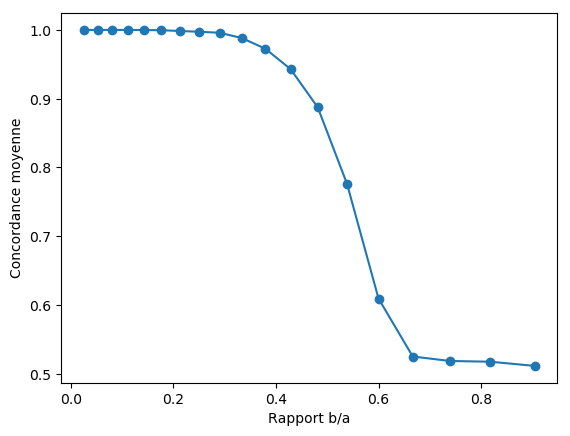
\includegraphics[scale=0.85]{evol_mean_concordance.png}
    \caption{Évolution de la concordance en fonction du rapport $b/a$, en utilisant Metroplis-Hastings}
    \label{conco}
\end{figure}\\
On remarque que plus $A$ et $B$ sont écartés, donc plus $b/a$ est petit, plus la concordance est élevée et, inversement, plus cette écart diminue, moins il est facile de détecter des communautés.\\

Cela est dû au fait que l'algorithme de Metropolis-Hastings se base sur la détection d'ensembles de noeuds qui comportent beaucoup d'arêtes communes. Étant donné que $A$ et $B$ sont, respectivement, les probabilités que des noeuds d'une même communauté soient connectés et que des noeuds de communautés différentes soient connectés. Par conséquent, plus $A$ et $B$ diffèrent, meilleur est l'algorithme car les différents groupes de noeuds sont bien délimités. À contrario, plus $A$ et $B$ se rapprochent, moins bon sont les résultats. Prenons le cas où $A=B$, si ces deux probabilité sont égales, l'algorithme de Metropolis-Hastings ne détectera jamais de communautés distinctes, puisqu'il y a autant de liens intra-communautés que de liens entre communautés différentes. C'est donc pourquoi, l'algorithme de Metropolis-Hastings, utilisé ici, fonctionne mieux pour des graphes où $A>>B$, c'est-à-dire lorsque les noeuds sont plus connectés au sein d'une même communauté, et qu'il est dès lors possible de détecter ces communautés.
 
\subsubsection{Question 2}

On récupère maintenant les mêmes valeurs de $a$ et $b$ qu'à la section \ref{221} ainsi que les 10 graphes et vecteurs de communautés générés mais, cette fois-ci, à la place d'utiliser l'algorithme de Metropolis-Hastings on génère les estimations aléatoirement. La figure \ref{aleatoire} ci-dessous à droite montre l'évolution de la concordance moyenne en fonction de $b/a$ pour cette méthode.

\begin{figure}[h!]
    \begin{minipage}{.5\textwidth}
        \centering
        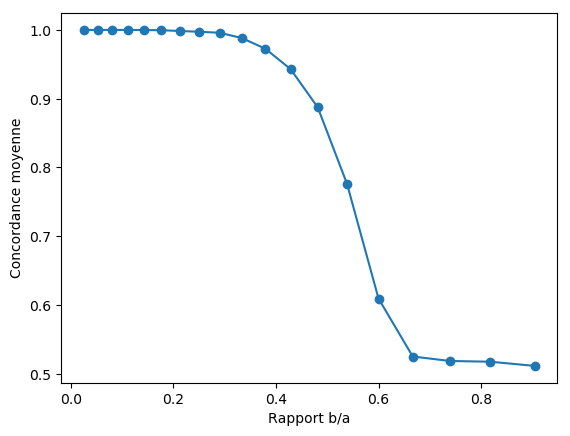
\includegraphics[width=8cm]{evol_mean_concordance.png}
        \caption{Évolution de la concordance en fonction du rapport $b/a$, en utilisant Metroplis-Hastings}
        %\label{conco}
    \end{minipage}
    \hspace{0.2cm}
    \begin{minipage}{.5\textwidth}
        \centering
        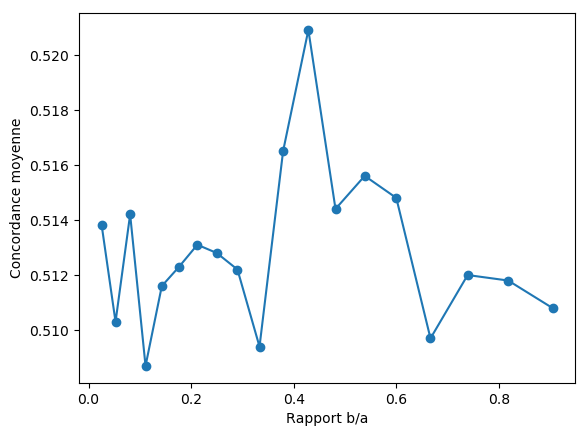
\includegraphics[width=8cm]{evol_random_mean_concordance.png}
        \caption{Évolution de la concordance moyenne en fonction du rapport $b/a$, en générant les vecteurs aléatoirement}
        \label{aleatoire}
    \end{minipage}
\end{figure}\\\\

Ces résultats sont en adéquation avec ceux présentés dans la littérature.\cite{Sweets} \cite{Demaine2007} En effet, on remarque que le phénomène de transition de phase est bien présent : lorsque $N$ tend vers l’infini et que $A=a/N$ et $B=b/N$ les communautés peuvent être détectées de manière plus précise que par une méthode purement aléatoire si et seulement si 
$$(a-b)^2 > 2(a+b)$$
Dans notre cas, avec un degré moyen $\frac{a+b}{2}$ fixé à 20, c'est bien après le rapport $\frac{b}{a} = 0.6$ (correspondant à $b=15$ et $a=25$ donc $100 > 80$), dernière valeur respectant l'inégalité, que la concordance chute et qu'elle n'atteint plus que des scores semblables à ceux obtenus à l'aide d'une méthode aléatoire. Avant et jusqu'à ce palier, les résultats sont bien meilleurs.\\

\newpage

\subsection{Application à un grand graphe}
Premièrement, pour éviter tout problème d'instabilité numérique lié à la manipulation de décimales extrêmement petites lors du calcul de $P(vector)$ et de $P(G|vector)$ (avec $vector = x$ ou $vector = y$), on fait le choix de réaliser nos opérations en logarithmes. Cela permet de transformer les produits en sommes.\\
% Ainsi, les résultats obtenus sont les plus fidèles possibles.

Ensuite, dans l'optique d'optimiser la précision de l'algorithme il est important de pouvoir réaliser un grand nombre d'itérations et, pour ce faire, il faut absolument réduire le temps nécessaire à l'exécution du code.\\

Deux opérations sont fortement chronophages car nécessitant de parcourir l'entièreté du grand graphe pour la première, et l'entièreté du vecteur estimation pour la seconde. Ces opérations sont  le calcul du nombre d'arêtes entre chaque paire de communautés et le calcul du nombre de noeuds présents dans chaque communauté.\\

Pour y remédier, on crée pour chacune de ces valeurs une matrice destinée à stocker ces informations en mémoire, celles-ci étant calculées une et une seule fois en amont de l'exécution de l'algorithme. Ces 2 tableaux sont ensuite mis à jour au fur et à mesure des itérations en évitant donc de parcourir à chaque fois l'entièreté du grand graphe et l'entièreté du vecteur estimation. A noter que les matrices sont mise à jour uniquement si le vecteur candidat $y$ est accepté. Dans le cas contraire, on passe à l'itération suivant sans modifier les informations en mémoire.\\

Afin d'obtenir de bons résultats lors de la compétition, on doit utiliser l'algorithme de Metropolis-Hastings avec un nombre d'itérations suffisamment grand. On a choisit 200 000 itérations en vue de réduire le plus possible le facteur chance de l'algorithme tout en restant raisonnable au niveau du temps d'exécution. Dans ces conditions on est donc certain de trouver une concordance élevée ($ >90\% $) ainsi qu'un temps de calcul raisonnable ($< 2h$). Dans cette configuration, on a atteint $93.84\%$ de concordance et l'exécution a pris $\approx 1h30$.\\

\newpage
\bibliographystyle{plain}
\bibliography{bib_stocha.bib}
\end{document}